Esta Seção aborda os resultados obtidos através das respostas coletadas nos questionários citados na Seção 4.3. Uma análise descritiva foi feita com as respostas do questionário fechado dos professores e também com o aberto dos alunos devido ao baixo número de respostas. Como o questionário fechado dos alunos foi o artefato central desta pesquisa, foram realizadas duas análises: uma análise fatorial confirmatória, a fim de examinar os resultados obtidos a partir de duas perspectivas complementares, e uma análise descritiva, a fim de examinar se houve diferença na média das avaliações causada por diferença de níveis de experiência dos alunos.

\subsection{Análise dos questionários fechados dos professores}

Analisando as respostas dos questionários fechados dos seis professores participantes, foi possível observar que sua percepção geral acerca das práticas foi a seguinte: i) os alunos apresentaram bom engajamento; ii) a complexidade das práticas variou entre baixa e média; iii) o desempenho dos alunos foi satisfatório; iv) os alunos apresentaram facilidade para realizar as práticas; v) as práticas tinham propostas alinhadas com a realidade do mercado de \textit{software}.

Os resultados observados a partir das respostas dos professores foram condizentes com aqueles observados nas demais análises feitas nesta Seção 5. Ademais, durante a aplicação das práticas, os pesquisadores notaram engajamento e participação ativa de todos os professores, que demonstraram interesse em colaborar com a pesquisa como conseguissem, interagindo com os pesquisadores e incentivando a participação dos alunos na pesquisa.

\subsection{Análise dos questionários abertos dos alunos}

Analisando as respostas dos questionários abertos dos alunos, foi possível observar em seus \textit{feedbacks} que ficaram satisfeitos com as práticas, no geral, apenas sinalizando que o tempo disponibilizado para a realização delas poderia ter sido maior. Entretanto, a duração das práticas nas aulas em que elas foram aplicadas foi pensada e negociada com os professores para que não se tomasse demasiado tempo de suas aulas -- o que poderia afetar negativamente o cronograma que já haviam planejado. 

Todavia, este resultado é coerente com os resultados dos questionários fechados dos alunos, que indicam que existem melhorias que podem ser feitas na adequação das práticas. Os níveis observados de satisfação geral e proximidade com o mercado também foram condizentes com aqueles observados na análise dos questionários fechados dos alunos.

\subsection{Análise dos questionários fechados dos alunos}

O experimento foi realizado em 5 disciplinas, somando 126 alunos, ao todo. Foram recolhidas 68 respostas nos questionários fechados das práticas, totalizando uma taxa de respostas correspondente a 53,9\% do número total de alunos matriculados nas disciplinas em que as experimentações foram realizadas. Levando em consideração que, para viabilizar o estudo proposto, seriam necessárias no mínimo 50 respostas, de acordo com Hair et al. (2009)\nocite{hair2009analise}, pode-se afirmar que a meta de respostas foi atingida, possibilitando o seguimento às análises propostas.

\subsubsection{Análise fatorial confirmatória}

A partir das respostas obtidas e da análise feita pelo algoritmo em R, foi possível observar que a satisfação dos alunos e a proximidade com o mercado apresentaram níveis satisfatórios. Em contrapartida, houve bastante divergência nas respostas acerca da adequação das práticas, indicando que esta precisa ser melhorada para cada contexto de aplicação, principalmente no quesito tempo. É possível explicar tal divergência pela diferença de nível de experiência entre os alunos participantes, visto que as práticas foram aplicadas de maneira igual em todas as disciplinas.

Tais afirmações foram feitas com base nos resultados da análise fatorial confirmatória realizada por meio do algoritmo (que encontra-se nos artefatos deste trabalho, vide Apêndice). O nível de significância $\alpha1$ utilizado neste estudo é de 0,05 (ou seja, o intervalo de confiança é de 95\%). Todavia, ainda poder-se-ia aceitar um valor $\alpha$ correspondente a 0,10 \cite{hair2009analise}. Observou-se que o Alfa de Cronbach das variáveis S e M apresentou valores superiores a 0.6, enquanto a variável A apresentou um valor negativo. A variável A também apresentou baixa confiabilidade composta, correspondente a 0.3, enquanto S e M apresentaram valores correspondentes a 0.8 e 0.9, respectivamente. Os valores exatos e os resultados encontram-se dispostos na Tabela 1. 

\begin{table}[!ht]
\centering
\begin{tabular}{|l|l|l|l|l|}
\hline
Variável Latente & Itens & \begin{tabular}[c]{@{}l@{}}Alfa de Cronbach\\ (\textgreater 0,6)\end{tabular} & \begin{tabular}[c]{@{}l@{}}Confiabilidade Composta\\ (\textgreater 0,6)\end{tabular} & Resultado \\ \hline
S                & $X_{1-3}$     & 0.79                                                                          & 0.818                                                                                & Aprovado  \\ \hline
A                & $X_{4-6}$     & -0.057                                                                        & 0.306                                                                                & Reprovado \\ \hline
M                & $X_{7-9}$     & 0.9                                                                           & 0.906                                                                                & Aprovado  \\ \hline
\end{tabular}
\caption{Avaliação de confiabilidade das variáveis. Fonte: autores}
\end{table}

Conclui-se que as variáveis de Satisfação (S) e Proximidade com Mercado (M) foram aceitas, apresentando valores estatisticamente comprovados. A variável de Adequação (A) apresentou valores baixos devido ao nível de inconsistência encontrado nas respostas. A partir disso, é possível interpretar que seria necessário ajustar algumas dimensões das práticas, como tamanho, tempo e nível de complexidade, de maneira orientada ao contexto das disciplinas, visando a obtenção de resultados mais coesos sobre as mesmas. As práticas foram regularizadas e não ajustadas a contexto justamente para que fosse possível analisar o impacto dessa padronização sobre a coleção diversa de participantes do experimento. Este impacto foi notado na variável latente de Adequação.

\begin{table}[!ht]
\centering
\begin{tabular}{|l|l|l|}
\hline
\multicolumn{1}{|c|}{\begin{tabular}[c]{@{}c@{}}Variáveis \\ Latentes\end{tabular}} & \multicolumn{1}{c|}{\begin{tabular}[c]{@{}c@{}}Variáveis\\ Observadas\end{tabular}} & \multicolumn{1}{c|}{Carga Fatorial} \\ \hline
                                                                                    & X1                                                                                  & 1.000                               \\ \cline{2-3} 
S =$\sim$                                                                           & X2                                                                                  & 1.612                               \\ \cline{2-3} 
                                                                                    & X3                                                                                  & 1.049                               \\ \hline
                                                                                    & X4                                                                                  & 1.000                               \\ \cline{2-3} 
A =$\sim$                                                                           & X5                                                                                  & -0.562                              \\ \cline{2-3} 
                                                                                    & X6                                                                                  & 0.940                               \\ \hline
                                                                                    & X7                                                                                  & 1.000                               \\ \cline{2-3} 
M =$\sim$                                                                           & X8                                                                                  & 1.207                               \\ \cline{2-3} 
                                                                                    & X9                                                                                  & 1.109                               \\ \hline
\end{tabular}
\caption{Carga fatorial das variáveis observadas. Fonte: autores}
\end{table}

A Tabela 2 exibe as relações entre as variáveis latentes e suas respectivas variáveis observadas, gerando, a carga fatorial das perguntas do questionário fechado dos alunos, citado na Seção 4.3.2. Observando os dados da tabela 1, eram esperados valores adequados na carga fatorial das variáveis $X_{1-3}$ e $X_{7-9}$. As perguntas referentes à variável latente de Adequação não foram capazes de representar o modelo e, portanto, as variáveis $X_{4-6}$ apresentaram valores na carga fatorial que não expressam uma relação com a respectiva variável latente. Para entender melhor como o \textit{script} obteve os resultados dessa carga, a fórmula utilizada encontra-se descrita abaixo:

$S  = \lambda_{S1} * X_{1} + \lambda_{S2} * X_{2} + \lambda_{S3} * X_{3}$

$M  = \lambda_{M1} * X_{7} + \lambda_{M2} * X_{8} + \lambda_{M3} * X_{9}$

A Tabela 3 contém os valores de correlação existentes entre as variáveis observadas e as latentes. A correlação existiu apenas entre a variável de satisfação e a de mercado, essas tendo um resultado de p \textless{ }0,05. Como a variável de adequação apresentou problemas no modelo, também era de se esperar a falta de correlação com a mesma.

\begin{table}[!ht]
\centering
\begin{tabular}{|l|l|l|}
\hline
Constructos     & Covariância & P-Valor \\ \hline
S $\sim$ $\sim$ A & 0.169       & 0.063   \\ \hline
S $\sim$ $\sim$ M & 0.543       & 0.000   \\ \hline
A $\sim$ $\sim$ M & 0.120       & 0.296   \\ \hline
\end{tabular}
\caption{Covariância das variáveis latentes. Fonte: autores}
\end{table}

Os resultados apresentaram uma forte correlação entre as perguntas referentes à satisfação dos alunos e também quanto à proximidade ao mercado, mostrando que o \textit{Lean Learning} pode ser uma metodologia de ensino que prepara melhor os alunos para as atividades comerciais de \textit{software}. Para melhorar ainda mais seu desempenho, precisaria se adequar melhor cada atividade prática para cada turma do curso, com base no nível de experiência esperado da turma, período e complexidade envolvida.

Além disso, notou-se uma forte correlação entre satisfação e mercado, visto que a correlação entre as variáveis apresentou um valor p = 0,03. Os pesquisadores observaram uma adesão maior dos alunos justamente às práticas 1 e 3, onde a comunicação era um dos temas principais das práticas. A prática 2, por se tratar de um exercício de lógica, aparentou entediar os alunos mais experientes do curso e assustar os mais novos, que não estariam tão preparados para ela. Acredita-se que com uma adequação melhor da prática, e um estímulo maior à competição, como recompensar mais pontos ou até mesmo recompensar o grupo vencedor com algum prêmio poderia resultar em maior participação, interesse e adequação na prática 2.

A Figura 4, trata-se do grafo de correlação entre as variáveis analisadas neste estudo. Este grafo foi gerado automaticamente ao final da execução do \textit{script} R e contém os valores de todas as variáveis discutidas nessa seção.

\begin{figure}[!ht]
    \centering
    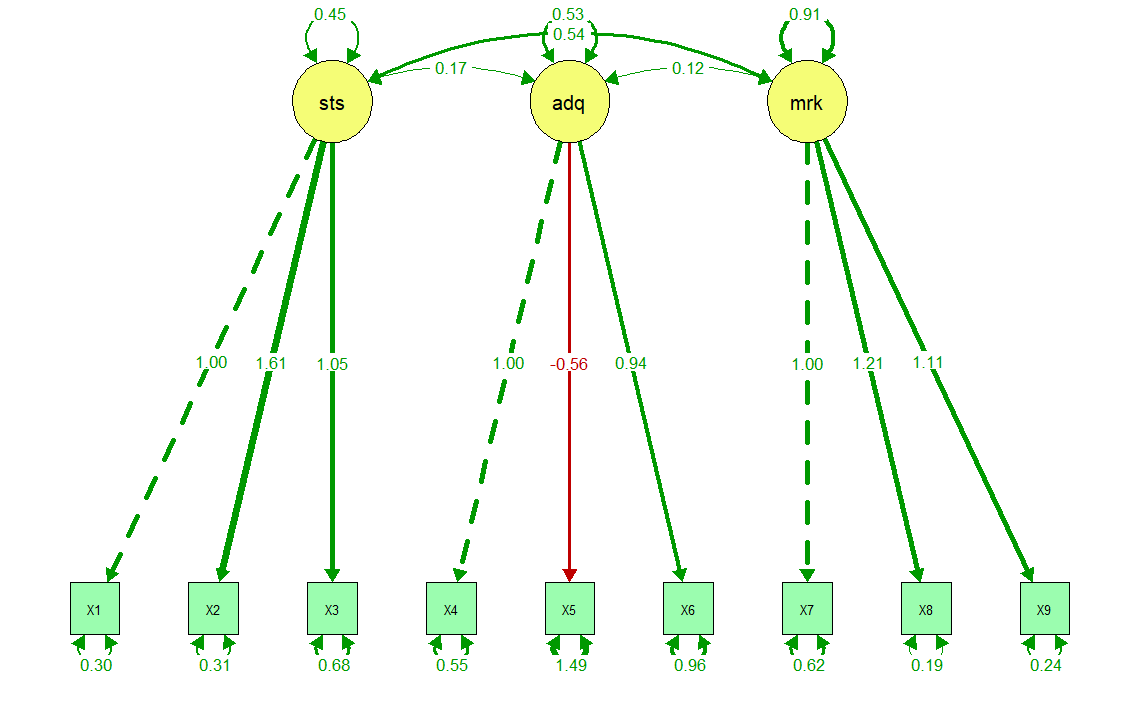
\includegraphics[width=15cm,height=8.5cm]{Imagens/RplotFinal.png}
    \caption{Grafo de correlação das variáveis. Fonte: autores}
    \label{fig:RplotFinal}
\end{figure}

\subsubsection{Análise descritiva}

Para a análise descritiva, os alunos foram divididos em dois grupos, de acordo com dados de triagem (considerados individualmente). No Grupo 1, encontram-se os alunos que: i) trabalham na área há 2 anos ou menos; ii) estão cursando o quarto período ou período menor; iii) têm 24 anos de idade ou menos. No Grupo 2, encontram-se os alunos que: i) trabalham na área há mais de 2 anos; ii) estão cursando o quinto período ou período maior; iii) têm mais de 24 anos de idade. A Tabela 4 mostra de forma numérica como a divisão dos alunos foi feita.

\begin{table}[!ht]
\centering
\begin{tabular}{|c|l|l|l|l|}
\hline
                                                                    & \multicolumn{1}{c|}{\begin{tabular}[c]{@{}c@{}}Condição\\ Grupo 1 (GP1)\end{tabular}} & \multicolumn{1}{c|}{\begin{tabular}[c]{@{}c@{}}Condição\\ Grupo 2 (GP2)\end{tabular}} & \multicolumn{1}{c|}{\begin{tabular}[c]{@{}c@{}}Contagem\\ Grupo 1\end{tabular}} & \multicolumn{1}{c|}{\begin{tabular}[c]{@{}c@{}}Contagem\\ Grupo 2\end{tabular}} \\ \hline
\begin{tabular}[c]{@{}c@{}}Tempo de trabalho\\ na área\end{tabular} & \textless{}= 2 anos                                                                   & \textgreater 2 anos                                                                   & 40                                                                              & 28                                                                              \\ \hline
Período no curso                                                    & \textless{}= 4º periodo                                                               & \textgreater 4º periodo                                                               & 12                                                                              & 56                                                                              \\ \hline
Idade                                                               & \textless{}= 24 anos                                                                  & \textgreater 24 anos                                                                  & 51                                                                              & 17                                                                              \\ \hline
\end{tabular}
\caption{Contagem de integrantes nos grupos. Fonte: autores}
\end{table}

A Tabela 5 exibe uma análise das médias das avaliações das variáveis latentes S e M para cada um dos grupos. A variável A foi desconsiderada, uma vez que não carregou fator e não apresentou valores consideráveis para a confiabilidade composta e o Alfa de Cronbach. Segundo esta análise, é possível verificar que os alunos do Grupo 1 -- menos experientes em termos de tempo de atuação na área e período da graduação e menos maduros em termos de idade -- identificaram maior relação entre as práticas realizadas e o mercado de trabalho e ficaram mais satisfeitos com sua participação nelas do que os alunos do Grupo 2, no geral.

Essa análise descritiva baseada em diferença de médias pode ser considerada estatisticamente válida, pois o cálculo até a mesma considera que o p-valor das variáveis S e M foi aceito mediante os resultados apresentados na Seção 5.3.1.

\begin{table}[!ht]
\centering
\begin{tabular}{|l|l|l|l|}
\hline
\multicolumn{1}{|c|}{\begin{tabular}[c]{@{}c@{}}Média S\\ GP1\end{tabular}} & \multicolumn{1}{c|}{\begin{tabular}[c]{@{}c@{}}Média M\\ GP1\end{tabular}} & \multicolumn{1}{c|}{\begin{tabular}[c]{@{}c@{}}Média S\\ GP2\end{tabular}} & \multicolumn{1}{c|}{\begin{tabular}[c]{@{}c@{}}Média M\\ GP2\end{tabular}} \\ \hline
4,1                                                                         & 3,9                                                                        & 3,7                                                                        & 2,9                                                                        \\ \hline
4                                                                           & 3,8                                                                        & 3,6                                                                        & 2,8                                                                        \\ \hline
4                                                                           & 3,3                                                                        & 3,6                                                                        & 4,2                                                                        \\ \hline
\end{tabular}
\caption{Média obtida por cada grupo nas variáveis latentes. Fonte: autores}
\end{table}